\section{Discrete Maps}


As shown in section 2, ECA that are allowed to grow infinitely in size can exhibit non-periodic and chaotic behavior, even though they are completely deterministic.   In this section we will only consider CA with a fixed number of cells per time step.  For this case, we must apply either fixed or periodic boundary conditions on the endpoints.  Here we use periodic boundary conditions and the phase space morphs from an infinite 1D lattice to a finite circular lattice.  For an ECA of finite width, n, there exists $2^n$ possible configurations (each site takes one of two values).  This means that every initial condition will eventually end in a periodic loop, although the period could be as large as $2^n -1$.  

We follow the methods of~\cite{sed} to convert the graphical ECA rules into discrete 1D maps.  In the same way each rule is labeled by a binary number, each time step in our finite ECA may be converted from binary into a base-10 number.  We wrote a \textsc{C++} code to loop over all $2^n$ possible configurations and record the resulting configuration after one time step (both are recoded in base 10).  We now have a 1D discrete map, mapping all the integers [0, $2^n -1$] $\rightarrow$ [0, $2^n -1$] for a given ECA rule.  With this mapping we can now iterate, either using cobweb diagrams or computer routines, to see the evolution as a function of time step.  The resulting maps are shown in Figures~\ref{30map} and~\ref{126map}.  The densely filled area is a result of connecting all the points in the map.  Figure~\ref{30map_dot} shows the same figure without the  lines connecting successive points.  

\begin{figure}
    \begin{minipage}[b]{0.49\textwidth}
        \centering
        \includegraphics[width=\textwidth]{30map.eps}
        \caption{\label{30map} The mapping for rule 30, using a grid width of 10 lattice points.  }
    \end{minipage}
    \hspace{0.5cm}
    \begin{minipage}[b]{0.49\textwidth}
        \centering
        \includegraphics[width=\textwidth]{30map_dot.eps}
        \caption{\label{30map_dot} The mapping for rule 30, shown without the connecting lines between points.}
    \end{minipage}
\end{figure}

The resulting maps are much more complicated in appearance than any of the maps we studied during the semester, such as the chaotic logistic map.  The large difference from continuous maps is that the axises are discrete so there is no possibility of rounding error or computer dependent results.  Adding more lattice points to the map results in the same structure, but with a higher resolution.  This is shown in Figures~\ref{126map_6} and~\ref{126map} where the lattice size is varied from six to ten points.  The alternating behavior between points differing by 512 and results in the filled region of the map can be clearly seen with the six site map.  

\begin{figure}
    \begin{minipage}[b]{0.49\textwidth}
        \centering
        \includegraphics[width=\textwidth]{126map_6.eps}
        \caption{\label{126map_6} The mapping for rule 126 using a width of 6 lattice points.  }
    \end{minipage}
    \hspace{0.5cm}
    \begin{minipage}[b]{0.49\textwidth}
        \centering
        \includegraphics[width=\textwidth]{126map.eps}
        \caption{\label{126map} The mapping for rule 126 using a width of 10 lattice points.}
    \end{minipage}
\end{figure}

By iterating these maps we can look at the growth of the system as a function of time step.  As previously mentioned, all initial conditions will eventually reach a periodic cycle.  Figure~\ref{30iter_IC32} shows the growth of rule 30 over 1,000 iterations with initial condition 32 (one black block).  This system hits a stable period-15 cycle after 7 iterations.  Figure~\ref{30iter_IC33} shows the same evolution of rule 30, but now with initial condition 33.  These two initial conditions only differ by one bock, but the system now hits a period-5 cycle immediately after starting.  Even though the initial conditions may not be continuously varied in these discrete systems, there is still a strong sensitivity to initial conditions.  

\begin{figure}
    \begin{minipage}[b]{0.49\textwidth}
        \centering
        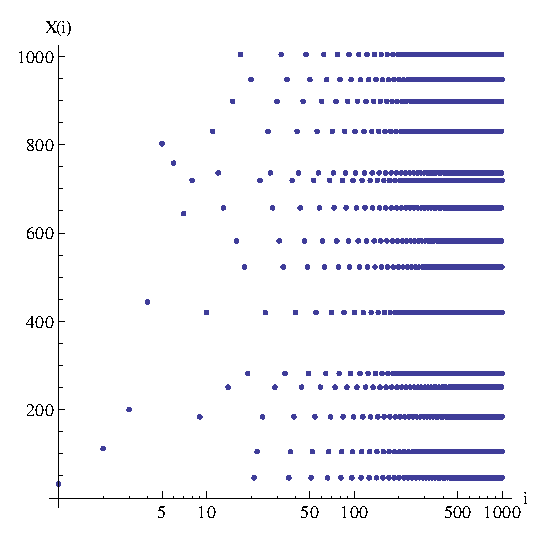
\includegraphics[width=\textwidth]{30iter_IC32.eps}
        \caption{\label{30iter_IC32} 1,000 iterations of rule 30 with an initial condition of 32.   }
    \end{minipage}
    \hspace{0.5cm}
    \begin{minipage}[b]{0.49\textwidth}
        \centering
        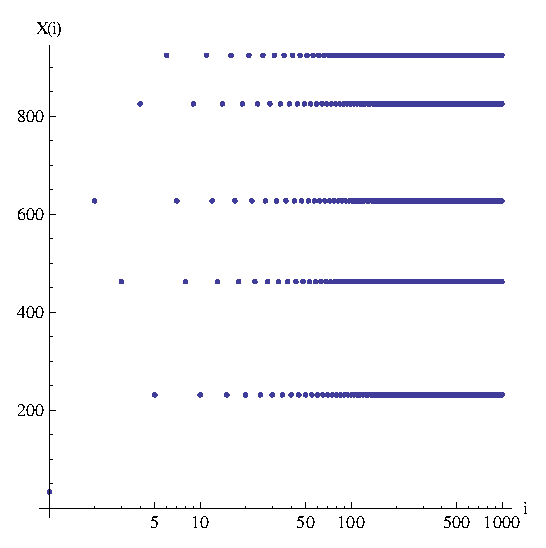
\includegraphics[width=\textwidth]{30iter_IC33.eps}
        \caption{\label{30iter_IC33} 1,000 iterations of rule 30 using the initial condition 33. }
    \end{minipage}
\end{figure}



